%%%%%%%%%%%%%%%%%%%%%%%%%%%%%%%%%%%%%%%%%%%%%%%%%%%%%%%%%%%%%%%%%%%%%%
%%                     Or
%%%%%%%%%%%%%%%%%%%%%%%%%%%%%%%%%%%%%%%%%%%%%%%%%%%%%%%%%%%%%%%%%%%%%%
%\color{blue}
\subsubsection{Glyph: \glyph{Or}}\label{sec:or}

The glyph \glyph{or} is used to denote that any of the \glyph{entity nodes} linked as input is sufficient to produce the output influence.

\begin{glyphDescription}

 \glyphSboTerm SBO:0000174 ! or.

 \glyphContainer \glyph{Or} is represented by a circle, with two connectors located at the opposite side for inputs and output.

  \glyphLabel \glyph{Or} is identified by the label ``OR'' placed in an unbordered box attached to the center of the container. 

  \glyphAux \glyph{Or} does not carry any auxiliary items.

\end{glyphDescription}

\begin{figure}[H]
  \centering
  \includegraphics[scale = 0.5]{images/or}
  \caption{The \ER glyph for \glyph{or}. Three inputs are represented, but two or more than three would be allowed.}
  \label{fig:or}
\end{figure}


\begin{figure}[H]
  \centering
  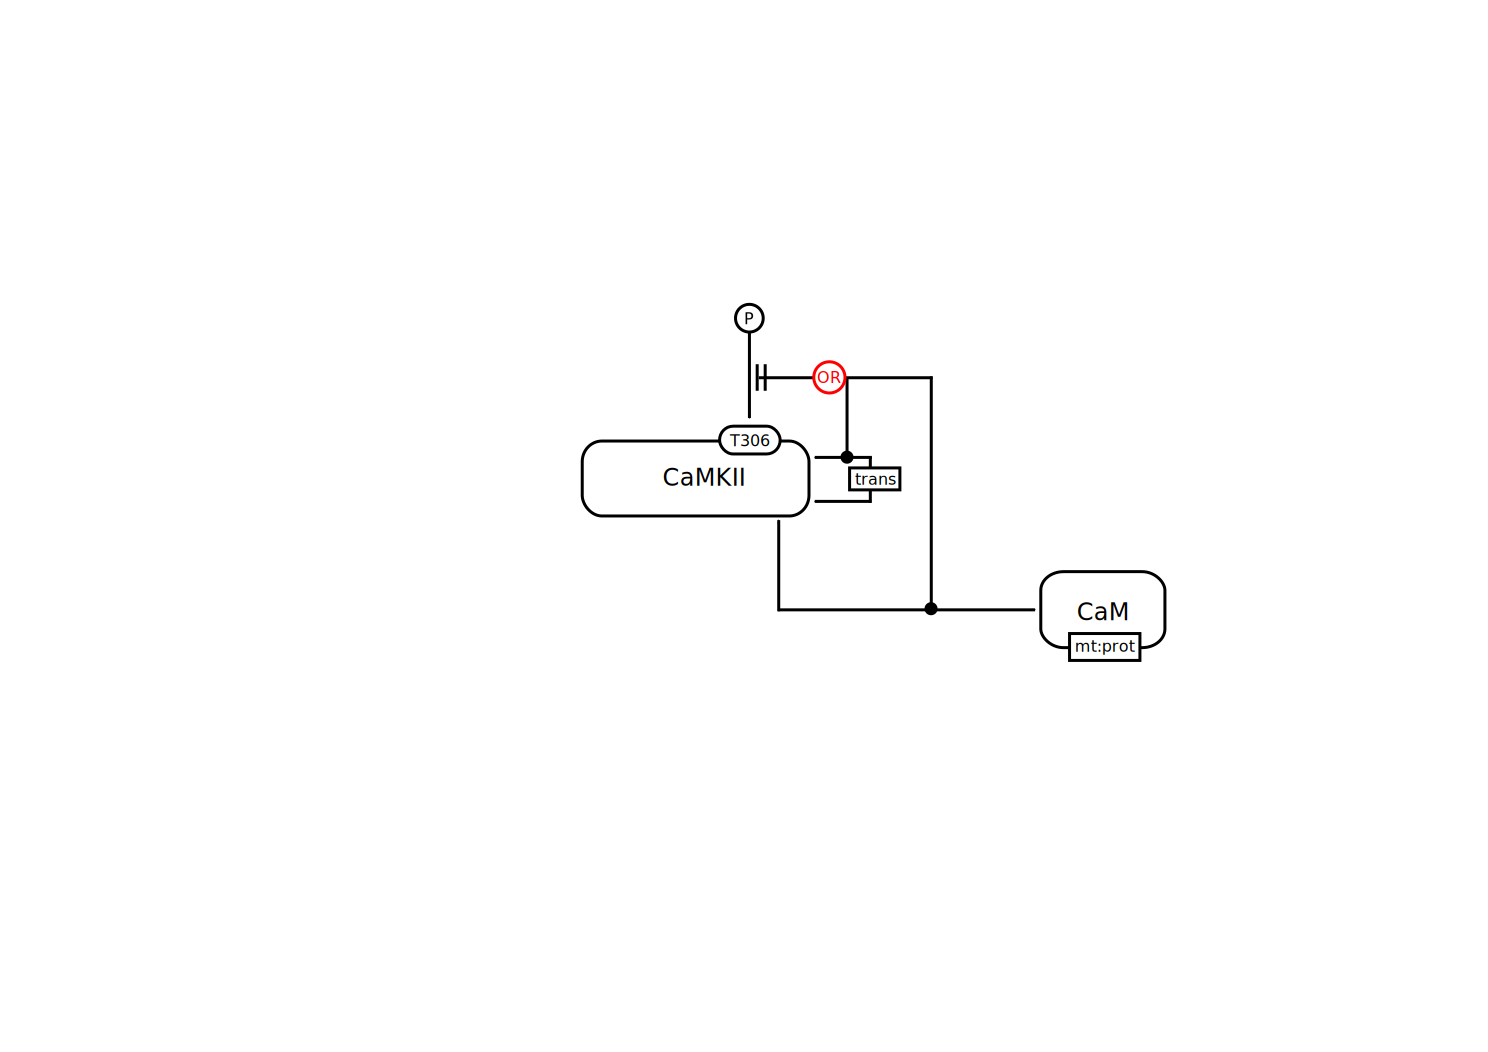
\includegraphics[scale = 0.5]{examples/ex-or}
  \caption{Example of the \glyph{or} logical operator, showing that either the dimerisation of CaMKII or its binding to Calmodulin preclude the phosphorylation of threonin 306.}
  \label{fig:ex-or}
\end{figure}